\titre{}
\theme{fonctions}
\auteur{Nathan Scheinmann}
\niveau{1M}
\source{}
\type{serie}
\piments{2}
\pts{}
\annee{2425}

\contenu{
	\tcblower
	Déterminer l'équation des droites représentées ci-dessous.
\begin{center}
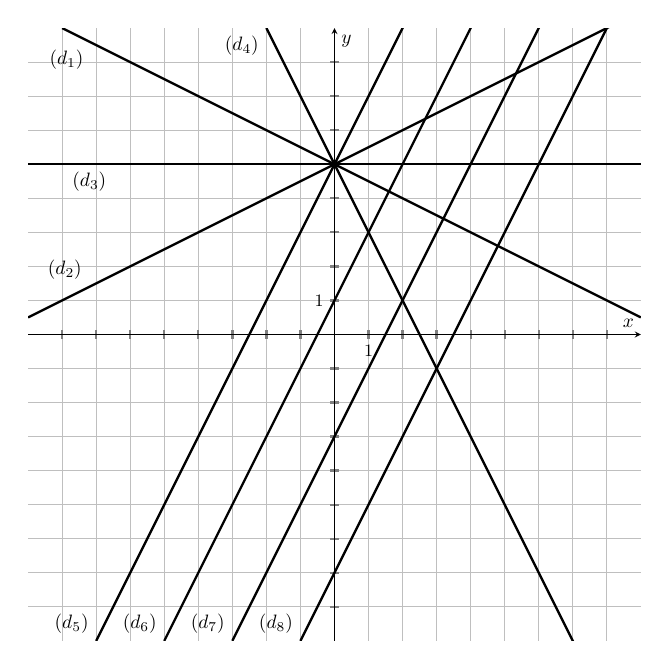
\begin{tikzpicture}[scale=0.7]
\begin{axis}[
  axis lines=center,
  grid=major,
  width=5in,
height=5in,
  xmin=-8,
  xmax=8,
  ymin=-8,
  ymax=8,
  xlabel=$x$,
  ylabel=$y$,
  enlargelimits={abs=1},
  xtick={-8,-7,...,8},
  ytick={-8,-7,...,8},
  xticklabels={,,,,,,,,0,1,,,,,,,},
  yticklabels={,,,,,,,,,1,,,,,,,},
  xlabel style={at={(rel axis cs:1,0.5)}},
  ylabel style={at={(rel axis cs:0.5,1)}},
  tick style={very thick},
  ticklabel style={font=\small},
  legend style={
  at={(rel axis cs:1,1)},
  anchor=north west,
  draw=none,
  inner sep=0pt,
  fill=gray!10}
]

\addplot [very thick,domain=-5:9,samples=200] {2*x+1} node [above left,pos=0.0] {$(d_6)$};
\addplot [very thick,domain=-3:9,samples=200] {2*x-3} node [above left,pos=0.00] {$(d_7)$};
\addplot [very thick,domain=-1:9,samples=200] {2*x-7} node [above left,pos=0.0] {$(d_8)$};
\addplot [very thick,domain=-7:9,samples=200] {2*x+5} node [above left,pos=0.0] {$(d_5)$};
\addplot [very thick,domain=-9:9,samples=200] {0.5*x+5} node [above left,pos=0.1] {$(d_2)$};
\addplot [very thick,domain=-9:9,samples=200] {5} node [below,pos=0.1] {$(d_3)$};
\addplot [very thick,domain=-8:9,samples=200] {-0.5*x+5} node [below left ,pos=0.05] {$(d_1)$};
\addplot [very thick,domain=-2:9,samples=200] {-2*x+5} node [below left,pos=0.0] {$(d_4)$};
%\addlegendentry {$f(x)=...$};
%\addlegendentry{$g(x)=...$};
\end{axis}
\end{tikzpicture}
\end{center}	

}
\correction{
	\tcblower
	\begin{tasks}(4)
\task $d_1=-\dfrac{1}{2}x+5$
\task $d_2=\dfrac{1}{2}x+5$
\task $d_3=5$
\task $d_4=-2x+5$
\task $d_5=2x+5$
\task $d_6=2x+1$
\task $d_7=2x-3$
\task $d_8=2x-7$
\end{tasks}
}

